\documentclass[11pt]{article}
\usepackage[a4paper,margin=1in]{geometry}
\usepackage{mathtools, amsthm, amssymb, amsmath}
\usepackage{multicol}

\usepackage[style=numeric, sorting=none]{biblatex}
\addbibresource{MV.bib}

\usepackage{graphicx}
\graphicspath{{./picture/}}

\usepackage{subcaption}

\usepackage{tikz}
\usetikzlibrary{positioning}

\usepackage{rotating}

\newtheorem{definition}{Definition}
\newtheorem{example}{Example}

\title{Generating of Music Variations: Dynamical Systems Approach}
\author{Rajamangala University of Technology Thanyaburi\\Kanatsanun Sub-udom\\Wannasa Rianthong\\Patipan Somwong}
\begin{document}
\maketitle
\begin{abstract}
This research introduces a novel approach to music composition aimed at mitigating composer burnout. Leveraging chaotic systems, specifically the Lorenz Equation known for its sensitivity to initial conditions, the proposed method maps musical data onto this system. By introducing variations in initial values, the method generates unpredictable compositions, fostering creativity and fresh perspectives. 
\end{abstract}

\section{Introduction}
This research aims to address the prevalent issue of composer's burnout by introducing a novel approach to music composition utilizing chaotic systems. The proposed method leverages the Lorenz Equation, a chaotic system renowned for its sensitivity to initial conditions. By mapping musical data onto the Lorenz Equation and introducing variations in initial values, the method generates novel and unpredictable musical compositions, stimulating creativity and fostering fresh perspectives in music composition.

In reality, there are now many AI technologies that can create music. However, these technologies often require high computational resources, making them unable to run on devices with low processing power. Additionally, some AI music composition tools may produce music in limited styles. Well-known AI music generation platforms \cite{bonnici_music_2021} today include:

\begin{itemize}
\item Mubert: An online AI music composition platform that allows users to create music easily without musical knowledge.
\item Soundraw: An AI music creation tool that helps users quickly create background music for videos or games.
\item Boomy: An AI music composition app that helps users create and distribute music on streaming platforms.
\item AIVA: An AI assistant for music composition that helps users create music in various styles.
\item Musicity: An AI music creation tool that utilizes deep learning models to generate music. This research project proposes a new approach that reduces the use of computational resources and creates music in a more diverse range of styles.
\end{itemize}

\section{Literature Review}

\subsection{Chaotic System}
Chaotic systems are like puzzles with clear rules, but tiny mistakes at the start (think a single misplaced piece) lead to wildly different solutions later on. Even though the rules are defined, the outcomes are unpredictable due to their sensitivity to initial conditions. This butterfly effect is seen in weather, fluid flow, and even some financial markets.

An example used in a Chaotic Systemg such as Modeling Natural Phenomena: Chaotic systems help model and understand various natural phenomena such as weather patterns, turbulent fluid flows, ecological systems, and population dynamics.\cite{may_simple_1976}
Finance and Economics: Chaotic dynamics are studied in finance and economics to model stock market fluctuations, economic cycles, and price dynamics, providing insights into the inherent unpredictability and nonlinear behavior of financial systems \cite{mandelbrot_variation_1962}
Biomedical Systems: Chaotic systems are used to model and understand complex biological systems, including neural networks, cardiac rhythms, and gene regulatory networks, aiding in diagnosis, treatment, and understanding of diseases \cite{izhikevich_neural_2000}.

\subsection{Lorenz Equation}
The Lorenz equation is commonly defined as three coupled ordinary differential equation like:
\begin{align*}
\dot{x} &= \sigma(y - x), \\
\dot{y} &= rx - y - xz, \\
\dot{z} &= xy - bz,
\end{align*}
where $x$, $y$ and $z$ are the variables, and $\sigma > 0$, $r > 0$ and $b > 0$ are parameters. \\
When the Lorenz equation's parameters are set to $\sigma = 10$, $r = 28$ and $b = \dfrac{8}{3}$, it shows chaotic behavior, as illustrated in Figure \ref{fig:LE}. The Lorenz equations \cite{lorenz_deterministic_1963} have been applied across various domains such as Modeling Fluid Flows:  A study by J.C. Sprott in Chaos and Stability in Nonlinear Analog Circuits (2003) \cite{tlelo-cuautle_analogdigital_2019} explores how the Lorenz system can be applied to model specific fluid flows. This demonstrates its use in understanding fluid dynamics beyond just atmospheric convection.\cite{petrzela_chaos_2022}.
Cryptography: The chaotic nature of the Lorenz system makes it a potential candidate for secure communication. A research paper by S. Baptista et al. titled "Lorenz System Parameter Determination and Application to Break the Security of Two-channel Chaotic Cryptosystems" (2006) explores this application. While this paper discusses limitations of specific implementations, it highlights the potential of the Lorenz system in cryptography \cite{orue_lorenz_2006}
Engineering Applications: The Lorenz equations can be used to model certain electrical and mechanical systems that exhibit chaotic behavior. For instance, a paper by A.A. Fathy in "Chaos, Solitons  Fractals" (2009) investigates the application of the Lorenz system to brushless DC motors \cite{ge_anti-control_2006}. This showcases the potential for the Lorenz system in analyzing and potentially controlling chaotic behavior in engineering systems.

\begin{figure}
\centering
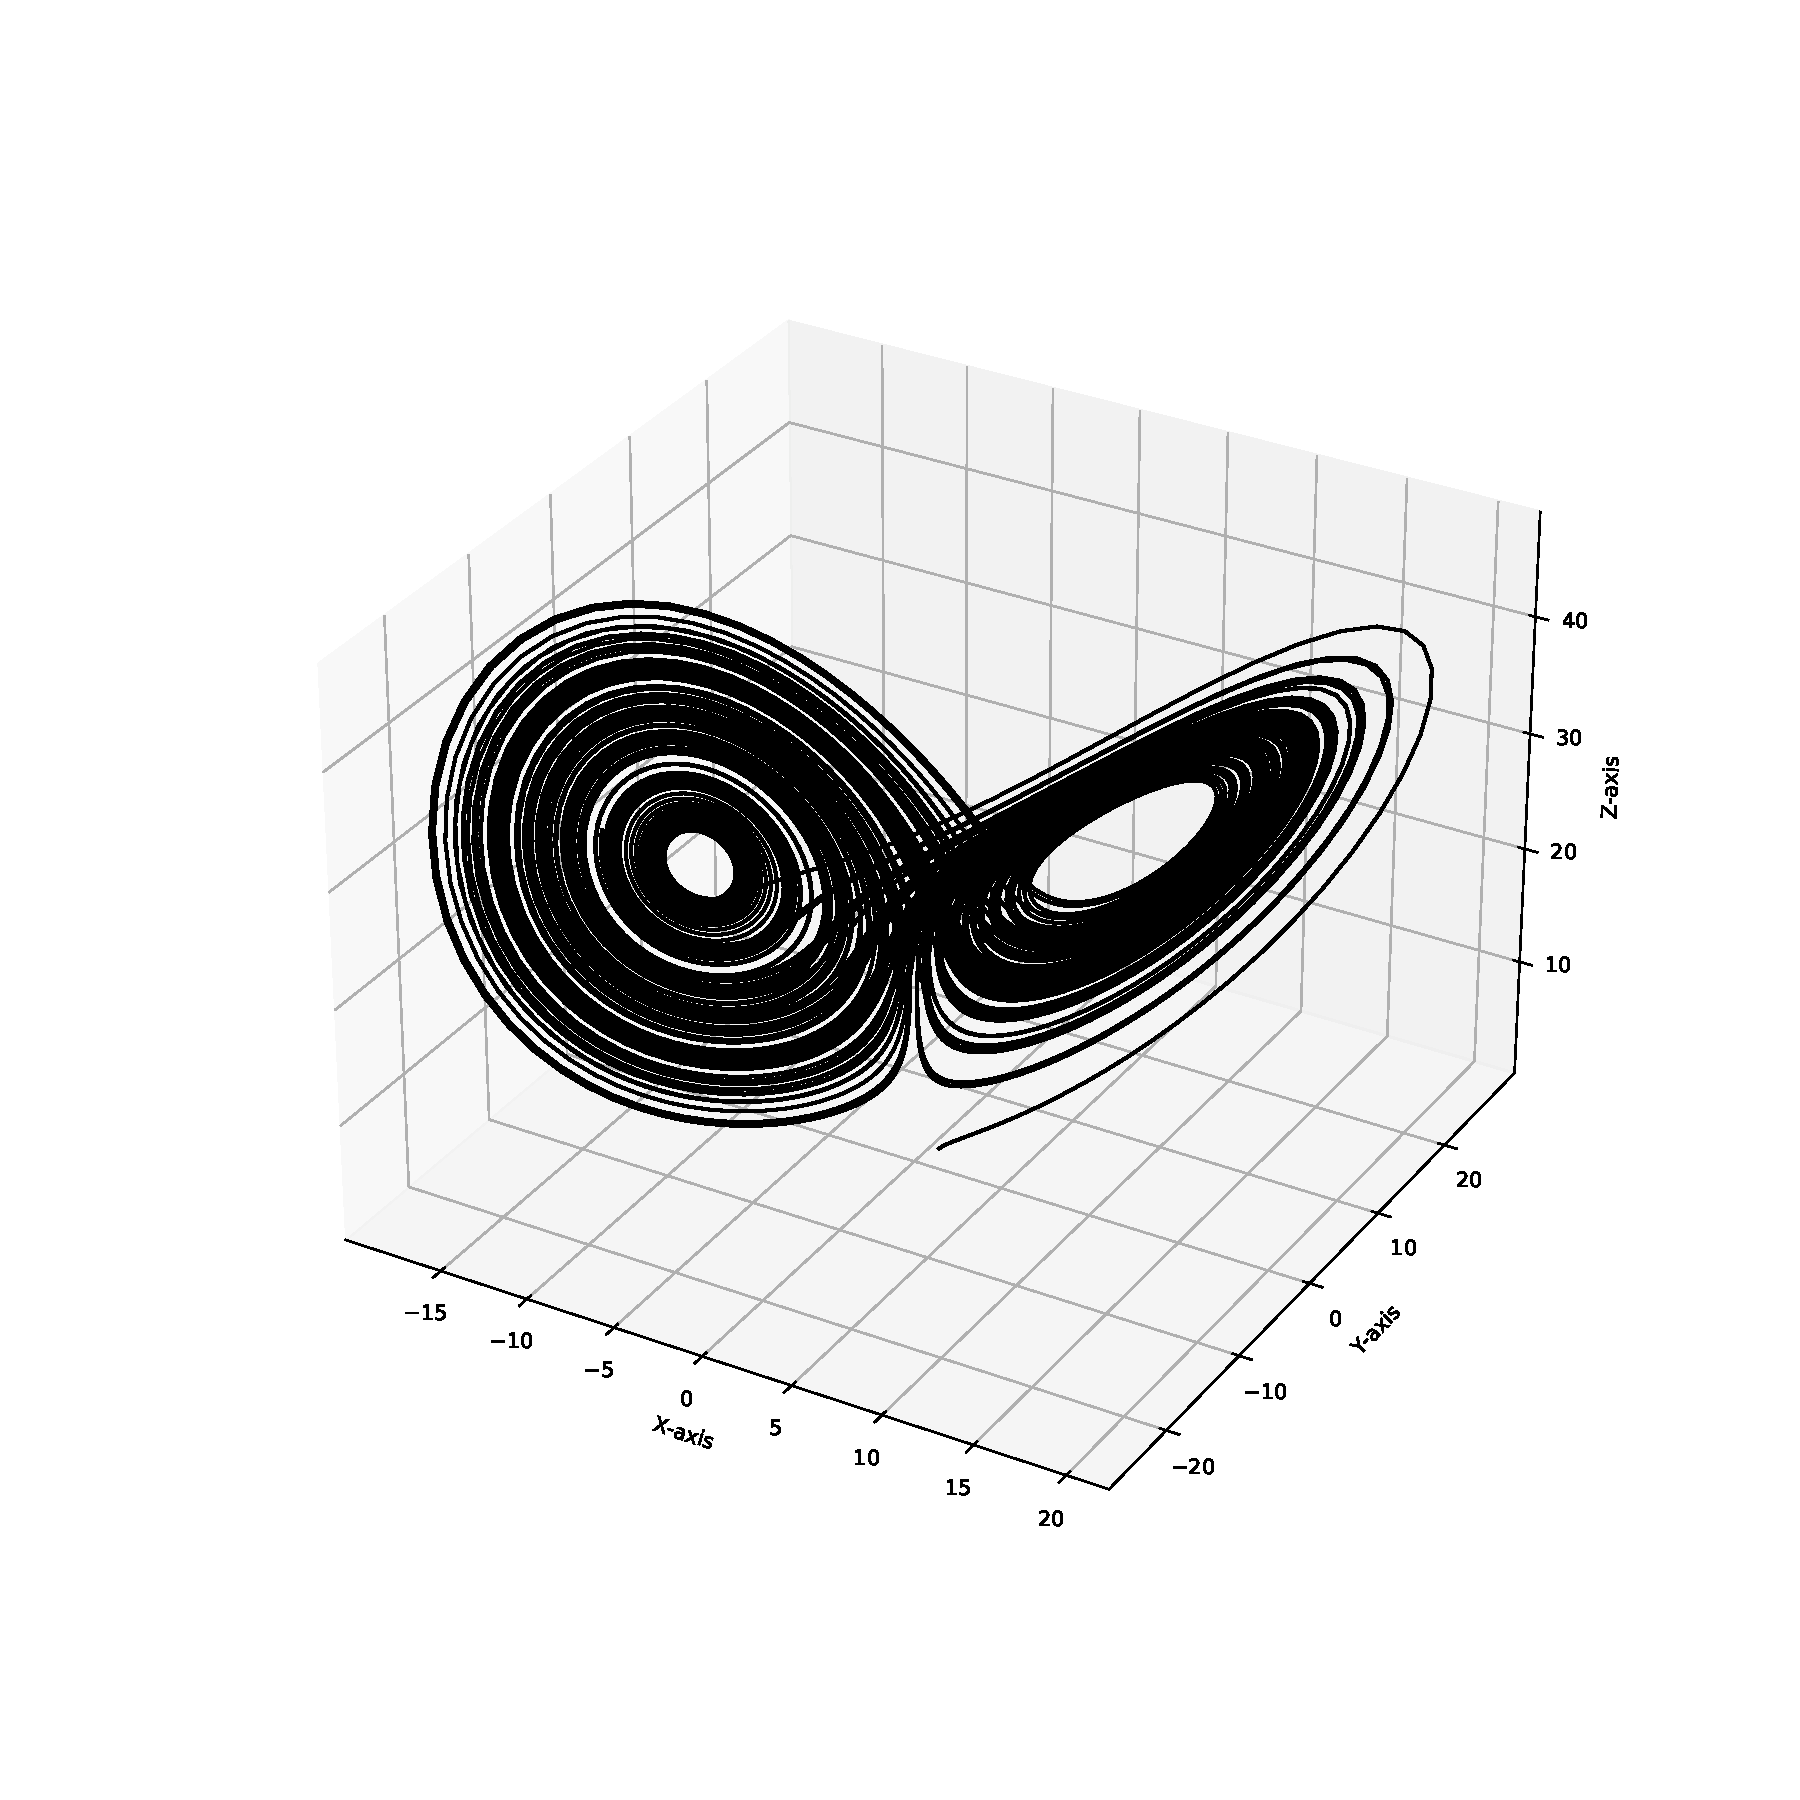
\includegraphics[trim=2cm 2cm 2cm 2cm, clip, scale=0.3]{Lorenz.pdf}
\caption{Chaotic behavior of the lorenz equation.}
\label{fig:LE}
\end{figure}

\subsection{Fourth-Order Runge–Kutta Implementation}
Let $\dot{y} = f(t,y)$. The approximation of $y_{i+1}$ is given by:
\begin{align*}
y_{i+1} &= y_i + \dfrac{h}{6}(k_1 + 2k_2 + 2k_3 + k_4), \\
k_1 &= f(t_i, y_i), \\
k_2 &= f\left( t_i + \dfrac{h}{2}, y_i + \dfrac{h}{2}k_1 \right), \\
k_3 &= f\left( t_i + \dfrac{h}{2}, y_i + \dfrac{h}{2}k_2 \right), \\
k_4 &= f(t_i + h, y_i + hk_3),
\end{align*}
\label{fig:RK4}
where $i = 0,1,2,...$ and $h$ is the step size, $y$ is the variable and $t$ is time. \\
The Runge-Kutta method \cite{bose_numerical_2019} is a powerful and popular family of numerical methods for approximating solutions to ordinary differential equations. These equations describe how a quantity changes with respect to another variable, but often cannot be solved exactly. The Runge-Kutta method tackles these problems by breaking down the interval of interest into smaller subintervals and iteratively calculating the solution at each subinterval. 

\subsection{Musical variations from a chaotic mapping: Diana S. Dabby}
Diana S. Dabby's research \cite{dabby_musical_1996} explores using chaotic systems to create musical variations. By leveraging chaotic trajectories' sensitivity to initial conditions, the study devises a method to introduce variability into a musical piece's pitch sequence. This allows for diverse musical variations while preserving the original composition's coherence. Dabby emphasizes the dynamic nature of this approach, offering composers a flexible tool for crafting a wide range of musical variations. Additionally, the study suggests extending this method beyond music to sequences of context-dependent symbols in various fields. Overall, the research showcases an innovative application of chaotic dynamics in music composition, yielding dynamic and versatile musical outcomes.

\subsection{Melodic Variation}
Melodic variation is essential in songwriting, adding depth and diversity to compositions. This article emphasizes its role in enhancing musicality and emotional depth. It cautions against monotony in melodies, stressing the importance of dynamic variation to engage listeners. Additionally, melodic variation contributes to a song's structure by creating contrast between sections. Two main methods are discussed: variations on a theme and countermelodies. Lastly, the article highlights the emotional impact of melodic variation and its ability to evoke a range of feelings in listeners. In conclusion, skillful use of melodic variation enables songwriters to craft compelling compositions that resonate deeply with audiences.

\section{Main Result}

This section explores the application of three techniques for generating musical variations, using the Ah vous dirai-je, Maman melody as a starting point and Lorenz Equation for chaotic
trajectory.

\subsection{Musical Variations from a Chaotic Mapping}

Let a sequence of pitches be represented by $P = \{p_1, p_2, \dots, p_n\}$. Let $\dot{x} = f(x)$ be a dynamical system with chaotic behavior. Then the approximate solution of $\dot{x}$ is denoted by $V = \{v_0, v_1, \dots, v_n\}$, when $v_0 \in \mathbb{R}_n$ is an initial condition of this trajectory. Let $K$ be a mapping from pitch to real value defined by 
$$K(p_i) = v_i.$$ 
Given $V^\prime = \{ v^\prime_1, v^\prime_2, \dots, v^\prime_n \}$ be a sequence of new trajectory by an initial condition of $v^\prime_0 \in \mathbb{R}_n$, where $v^\prime_0$ is started nearly $v_0$.

For each element $v^\prime$ in $V^\prime$, Let $L$ be a mapping from real value to pitch defines by 
$$L(v^\prime_i) = p_{j^*}.$$ 
Where $j^*$ is the chosen index for the new pitch according to the following criteria:
\begin{enumerate}
  \item If there exist the smallest $v_i$ such that $v_i > v^\prime_i$, then the new pitch must agree to use differ pitch, which is $j^* = j$ when $j$ is a index of a nearest $v_i$ value element such that $v_i > v_j$.
  \item If there exist a highest value $v^\prime_i$ such that $v_i < v^\prime_i$ for all $v_i$ in $V$, then the new pitch must agree to use highest $v_i$ value index. 
  \item If $v_i = v^\prime_j$, then the new pitch must agree to use the same pitch with the original pitch. 
  \item Otherwise, the new pitch must agree to use lowest $v_i$ value index.
\end{enumerate}
This creates a new sequence of pitches which can be represented by $\hat{P} =\{ \hat{p}_1, \hat{p}_2, \dots, \hat{p}_n \}$.

\begin{example}
Let a sequence of pitches of 12 variations on Ah vous dirai-je Maman in the first 3 bars in Figure \ref{fig:Dabby1} be represented by $P = \{C4, C4, G4, G4, A4, A4, G4, F4, F4, E4, E4 \}$. Let Lorenz system be a dynamical system with chaotic behavior by giving Lorenz parameters $r = 28, \sigma=10$ and $b = \frac{8}{3} $. Then the approximate solution of Lorenz system using fourth-order Runge–Kutta method with initial condition of $(1,1,1)$ is denoted by $X = \{1.00, 1.29, 2.13, 3.74, 6.54, 11.04, \\ 16.69, 19.56, 15.37, 7.55, 1.20\}$ when $X$ is sequence of x-value of approximate solution of Lorenz system. Let $K$ be a mapping from pitch to real value result as follows:

\begin{align*}
K(C4) &= 1.00, \\ 
K(C4) &= 1.29, \\
K(G4) &= 2.13, \\
K(G4) &= 3.74, \\
K(A4) &= 6.54, \\
K(A4) &= 11.04, \\
K(G4) &= 16.69, \\
K(F4) &= 19.56, \\
K(F4) &= 15.37, \\
K(E4) &= 7.55, \\
K(E4) &= 1.20. 
\end{align*}

Given $X^\prime = \{ 1.01, 1.30, 2.15, 3.76, 6.58, 11.10, 16.73, 19.55, 15.30, 7.48, 1.15 \}$ be a sequence of new trajectory with an initial condition of $(1.01,1,1)$ Let $L$ be a mapping from real value to pitch result as follows:
\begin{align*}
L(1.01) &= C4, \\
L(1.30) &= E4, \\
L(2.15) &= G4, \\
L(3.76) &= G4, \\
L(6.58) &= A4, \\
L(11.10) &= A4, \\
L(16.73) &= F4, \\
L(19.55) &= G4, \\
L(15.30) &= A4, \\
L(7.48) &= A4, \\
L(1.15) &= C4.
\end{align*}
This creates a new sequence of pitches which can be represented by $\hat{P} =\{C4, E4, G4, G4, A4, A4, \\ F4, G4, A4, A4, C4 \}$. Which can be converted to sheet music, as shown in Figure \ref{fig:Dabby2}. Since this method uses the same note duration and musical notes to create a new variation, so the resulting changes in the sequence compared to the original sequence might seem relatively small.
\end{example}

\begin{figure}
\centering
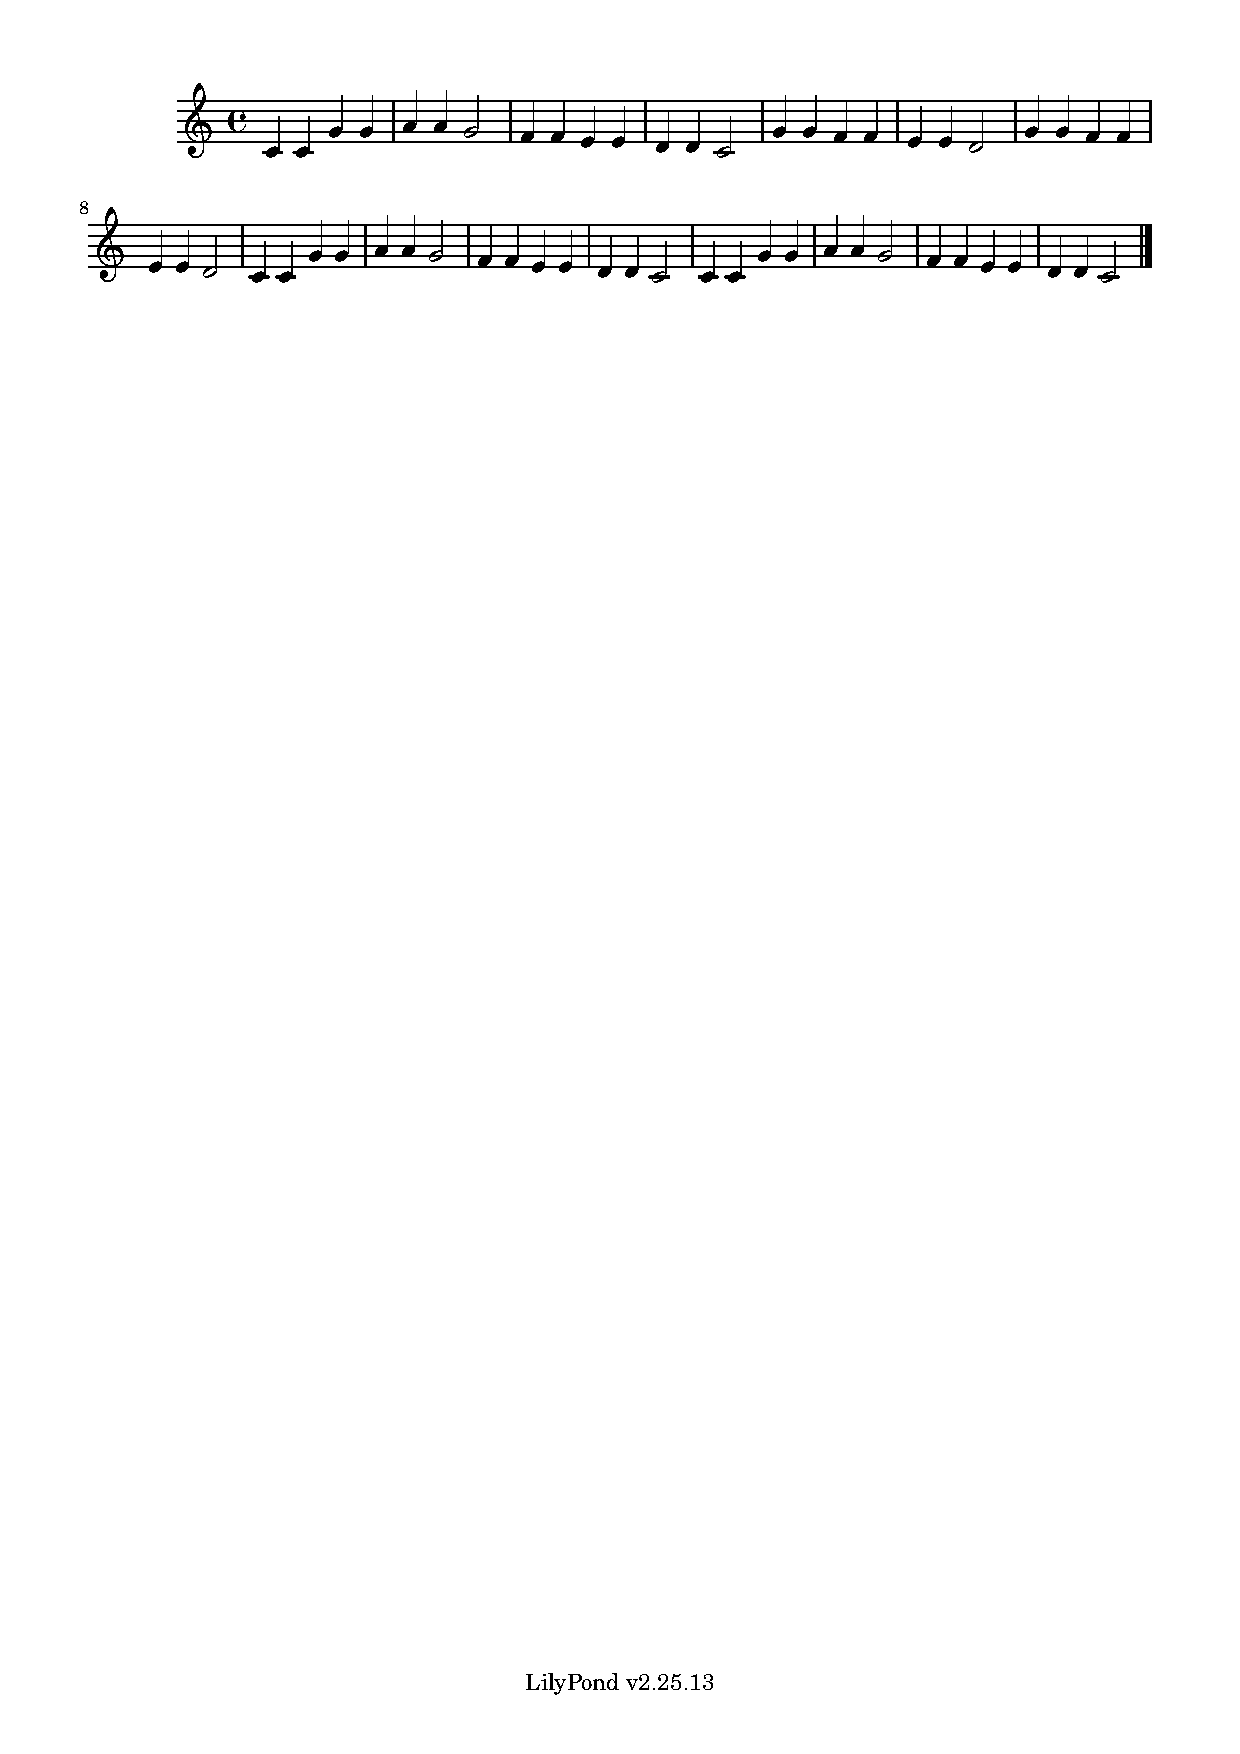
\includegraphics[trim=1cm 26.5cm 10.055cm 0.02cm, clip, scale=1]{dabby_1.pdf} % trim={left bottom right top}
\caption{The original of 12 variations on Ah vous dirai-je Maman in the first 3 bars.}
\label{fig:Dabby1} 
\end{figure}

\begin{figure}
\centering
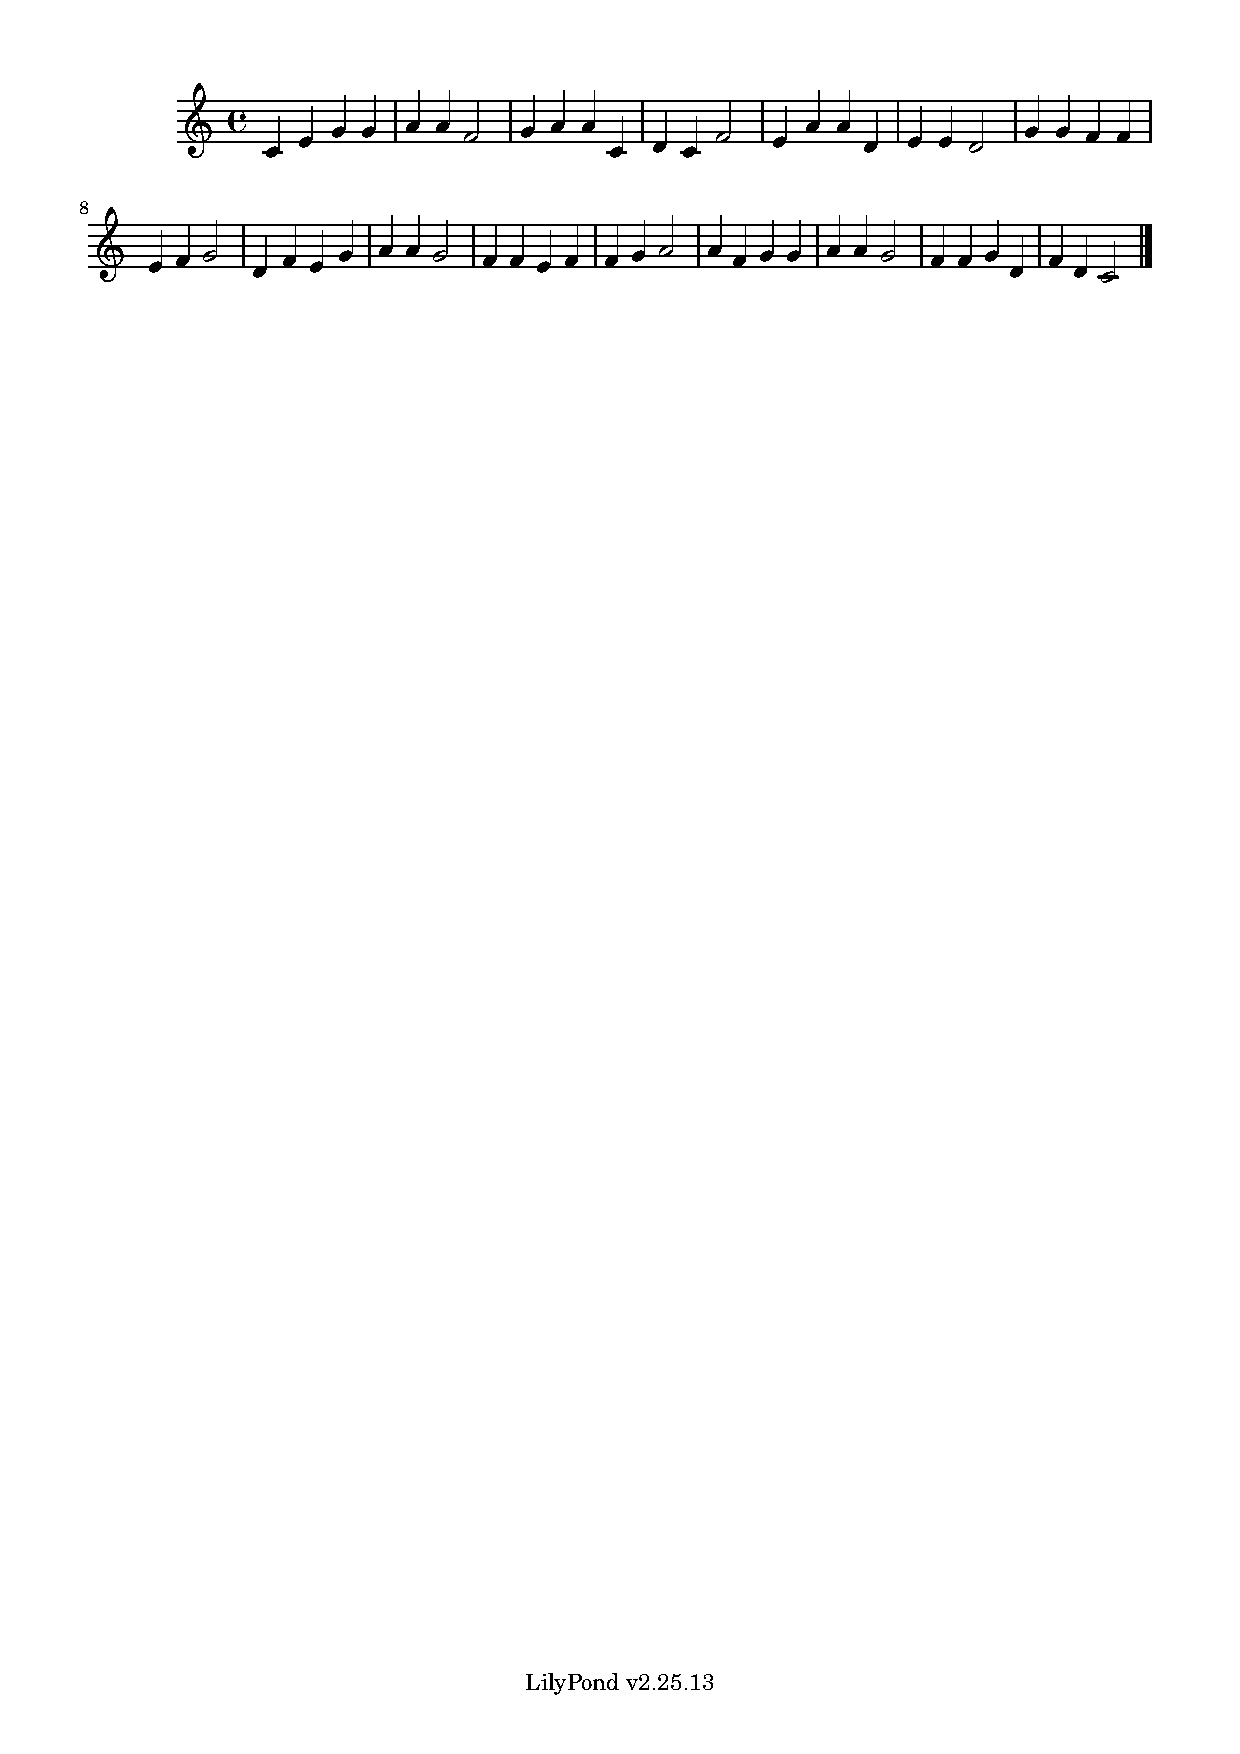
\includegraphics[trim=1cm 26.5cm 10.1cm 0.02cm, clip, scale=1]{dabby_2.pdf}
\caption{The new variation of Ah vous dirai-je, maman in the first 3 bars, generated by the Initial Condition $(1.01, 1, 1)$.}
\label{fig:Dabby2}
\end{figure}

\subsection{Melodic Variation with Expanded Rhythm Method} 
Given a note duration denoted by $\phi$ and divided into $D$ equal parts, the duration, $R$, of each individual division is defined by the following equation:
$$ R = \frac{\phi}{D}.  $$
\textbf{Note:} In musical theory, equal parts refers to divisions that all have the same duration.

\begin{example}
Consider the music piece 12 variations on Ah vous dirai-je Maman, illustrated in Figure \ref{fig:MV1}. The Figure shows that we already have 6 quarter notes and 1 half note.

If we want to divide each musical note into 4 parts, we can find the duration of each individual division as follows:
\begin{enumerate}
  \item[$\bullet$] Half note to 4 parts: $$R = \frac{\phi}{D} = \frac{2}{4} = 0.5$$
  \item[$\bullet$] Quarter note to 4 parts: $$R = \frac{\phi}{D} = \frac{1}{4} = 0.25$$
\end{enumerate}

Following this calculation, a half note can be divided into 4 eighth notes, and a quarter note can be divided into 4 sixteenth notes. This division is represented by the sequence \\ $P = \{C4, C4, C4, C4, C4, C4, C4, C4, G4, G4, G4, G4, G4, G4, G4, G4, A4, A4, A4, A4, A4, A4, \\ A4, A4, G4, G4, G4, G4 \}$ which can be converted to sheet music, as shown in Figure \ref{fig:MV2}.
\end{example}

\begin{figure}
\centering
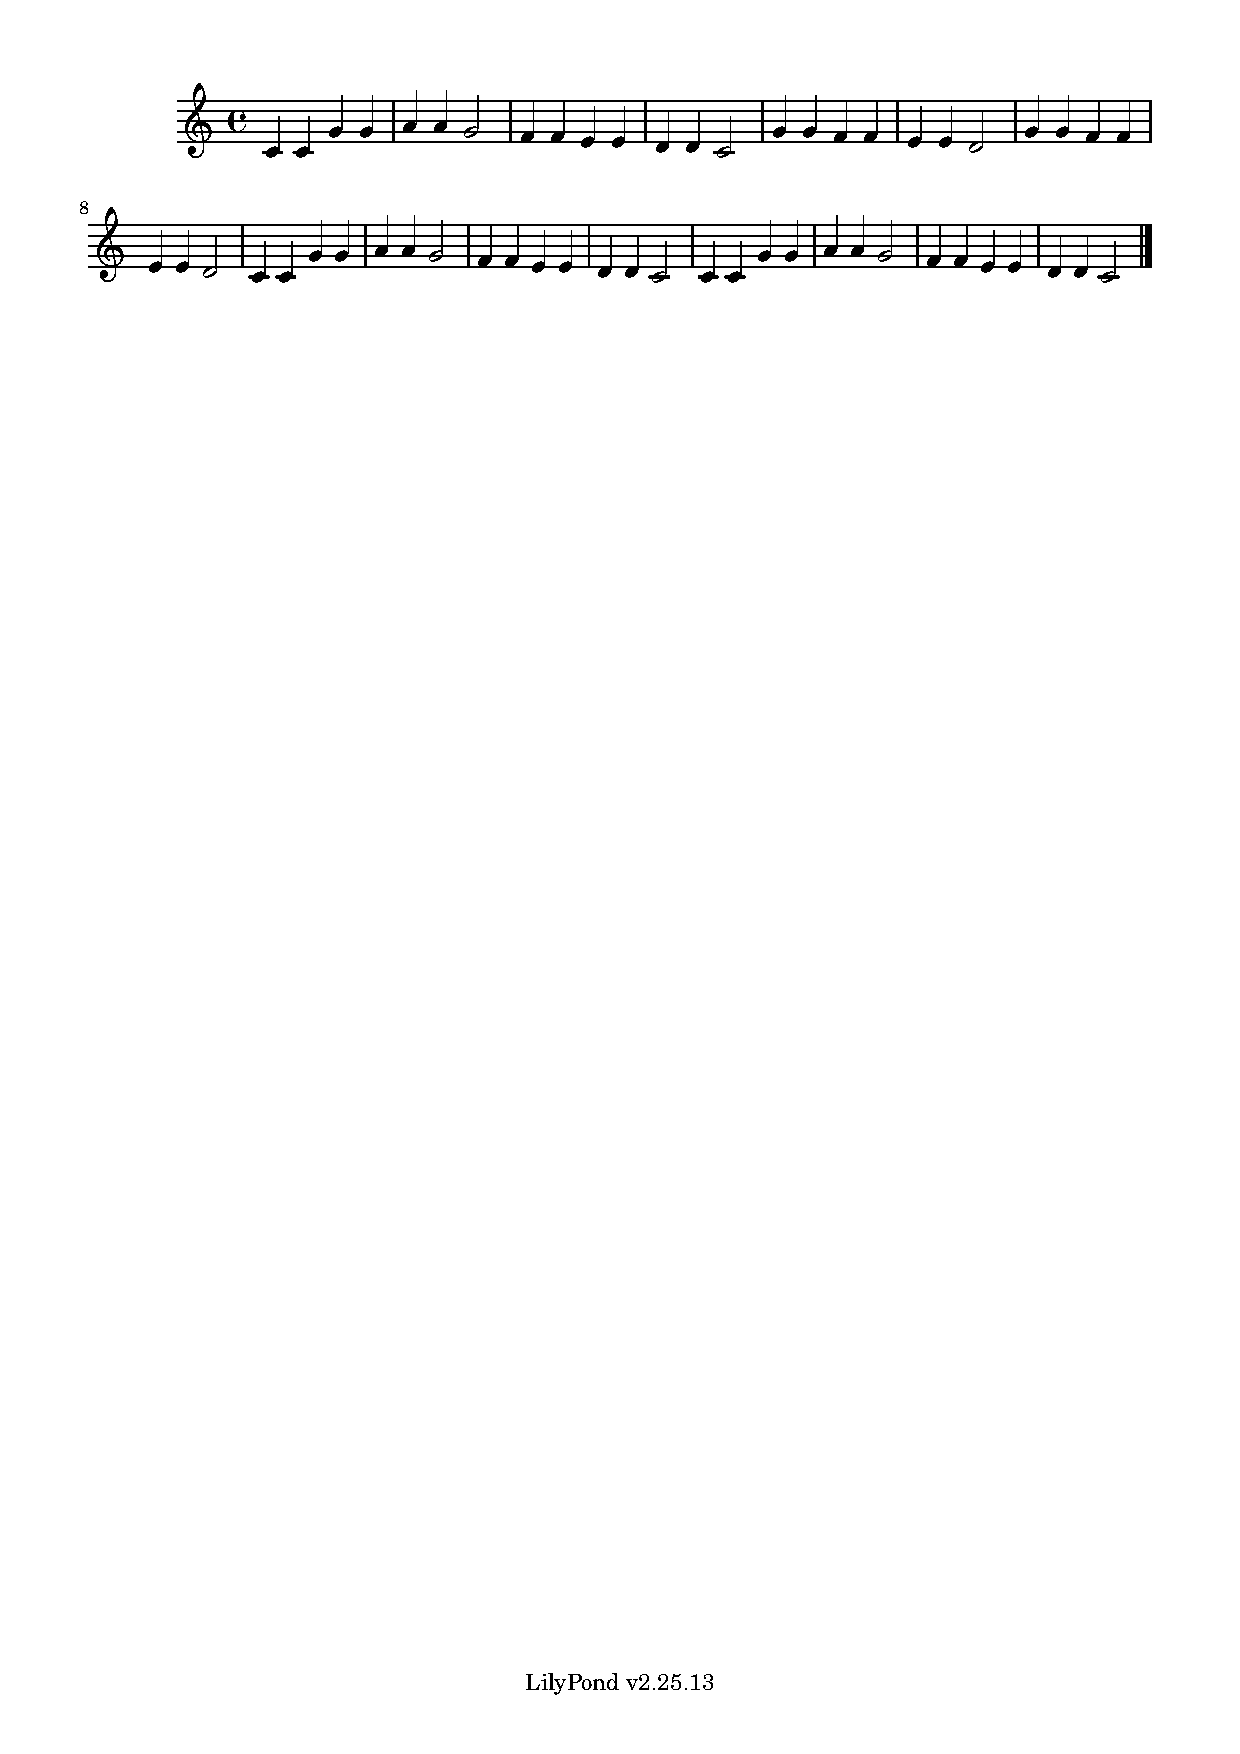
\includegraphics[trim=1cm 26.5cm 12.35cm 0.02cm, clip, scale=1]{dabby_1.pdf}
\caption{The original of 12 variations on Ah vous dirai-je Maman in the first 2 bars.}
\label{fig:MV1} 
\end{figure}

\begin{figure}
\centering
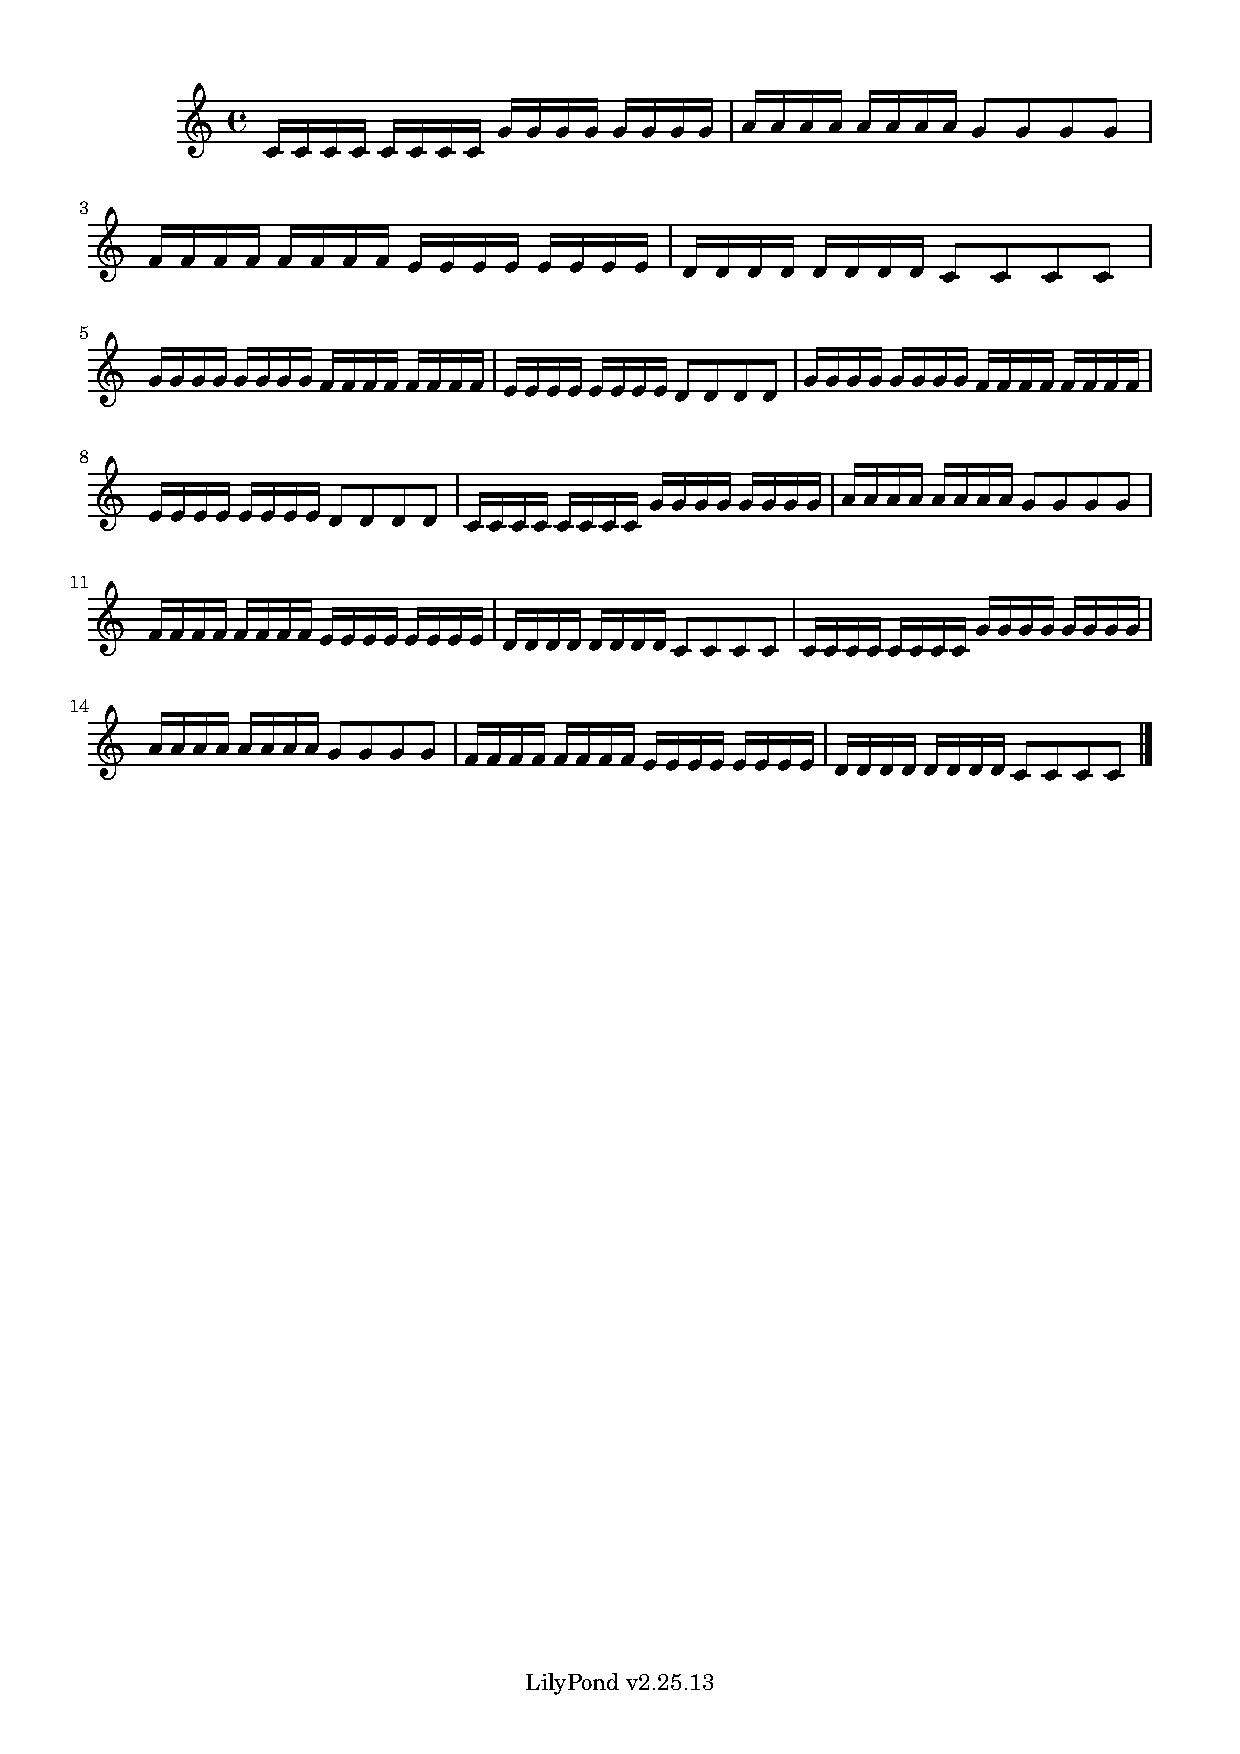
\includegraphics[trim=1cm 26.5cm 1cm 0.5cm, clip, scale=0.6]{melody_variation.pdf}
\caption{The melodic variation of Ah vous dirai-je, maman in the first 2 bars.}
\label{fig:MV2}
\end{figure}

\subsection{Combining Musical Variations from a Chaotic Mapping and Melodic Variation with Expanded Rhythm}
Let a sequence of pitches be represented by $P = \{p_1, p_2, \dots, p_n\}$ and a sequence of expanded rhythm pitches be represented by $P^* = \{p^*_1, p^*_2, \dots, p^*_n\}$. Let $\dot{x} = f(x)$ be a dynamical system with chaotic behavior. Then the approximate solution of $\dot{x}$ is denoted by $V = \{v_0, v_1, \dots, v_n\}$, when $v_0 \in \mathbb{R}_n$ is an initial condition of this trajectory. Let $K$ be a mapping from pitch to real value defined by 
$$K(p_i) = v_i.$$ 
Given $V^\prime = \{ v^\prime_1, v^\prime_2, \dots, v^\prime_n \}$ be a sequence of new trajectory with the same number of members as $P^*$ by an initial condition of $v^\prime_0 \in \mathbb{R}_n$, where $v^\prime_0$ is started nearly $v_0$.

For each element $v^\prime$ in $V^\prime$, Let $L$ be a mapping from real value to pitch defines by 
$$L(v^\prime_i) = p_{j^*}.$$ 
Where $j^*$ is the chosen index for the new pitch according to the following criteria:
\begin{enumerate}
  \item If there exist the smallest $v_i$ such that $v_i > v^\prime_i$, then the new pitch must agree to use differ pitch, which is $j^* = j$ when $j$ is a index of a nearest $v_i$ value element such that $v_i > v_j$.
  \item If there exist a highest value $v^\prime_i$ such that $v_i < v^\prime_i$ for all $v_i$ in $V$, then the new pitch must agree to use highest $v_i$ value index. 
  \item If $v_i = v^\prime_j$, then the new pitch must agree to use the same pitch with the original pitch. 
  \item Otherwise, the new pitch must agree to use lowest $v_i$ value index.
\end{enumerate}
This creates a new sequence of pitches which can be represented by $\hat{P} =\{ \hat{p}_1, \hat{p}_2, \dots, \hat{p}_n \}$.

\begin{example}
Let a sequence of pitches of 12 variations on Ah vous dirai-je Maman in the first 2 bars in Figure \ref{fig:MV1} be represented by $P = \{C4, C4, G4, G4, A4, A4, G4 \}$ and a sequence of expanded rhythm pitches on Figure \ref{fig:MV2} be represented by $P^* = \{C4, C4, C4, C4, C4, C4, C4, C4, G4, G4, G4, \\ G4, G4, G4, G4, G4, A4, A4, A4, A4, A4, A4, A4, A4, G4, G4, G4, G4 \}$. Let Lorenz system be a dynamical system with chaotic behavior by giving Lorenz parameters $r = 28, \sigma=10$ and $b = \frac{8}{3} $. Then the approximate solution of Lorenz system using fourth-order Runge–Kutta method with initial condition of $(1,1,1)$ is denoted by $X = \{1.00, 1.29, 2.13, 3.74, 6.54, 11.04, 16.69, 19.56, 15.37, 7.55, 1.20\}$ when $X$ is sequence of x-value of approximate solution of Lorenz system. Let $K$ be a mapping from pitch to real value result as follows:

\begin{align*}
K(C4) &= 1.00, \\ 
K(C4) &= 1.29, \\
K(G4) &= 2.13, \\
K(G4) &= 3.74, \\
K(A4) &= 6.54, \\
K(A4) &= 11.04, \\
K(G4) &= 16.69.
\end{align*}

Given $X^\prime = \{1.01, 1.30, 2.15, 3.76, 6.58, 11.10, 16.73, 19.55, 15.30, 7.48, 1.15, -2.70, -4.85, \\ -6.13, -7.06, -7.87, -8.64, -9.29, -9.70, -9.73, -9.37, -8.76, -8.07, -8.50, -7.17, -7.12, \\ -7.37, -7.85 \}$ be a sequence of new trajectory with an initial condition of $(1.01,1,1)$ Let $L$ be a mapping from real value to pitch result as follows:

\begin{multicols}{2}

\begin{align*}
L(1.01) &= C4, \\
L(1.30) &= C4, \\
L(2.15) &= G4, \\
L(3.76) &= G4, \\
L(6.58) &= A4, \\
L(11.10) &= A4, \\
L(16.73) &= A4, \\
L(19.55) &= G4, \\
L(15.30) &= A4, \\
L(7.48) &= A4, \\
L(1.15) &= C4, \\
L(-2.70) &= C4, \\
L(-4.85) &= C4, \\
L(-6.13) &= C4,
\end{align*}

\begin{align*}
L(-7.06) &= C4, \\
L(-7.87) &= C4, \\
L(-8.64) &= C4, \\
L(-9.29) &= C4, \\
L(-9.70) &= C4, \\
L(-9.73) &= C4, \\
L(-9.37) &= C4, \\
L(-8.76) &= C4, \\
L(-8.07) &= C4, \\
L(-8.50) &= C4, \\
L(-7.17) &= C4, \\
L(-7.12) &= C4, \\
L(-7.37) &= C4, \\
L(-7.85) &= C4.
\end{align*}

\end{multicols}
This creates a new sequence of pitches which can be represented by $\hat{P} = \{ C4, C4, G4, G4, A4, \\ A4, A4, G4, A4, A4, C4, C4, C4, C4, C4, C4, C4, C4, C4, C4, C4, C4, C4, C4, C4, C4, C4, C4 \}$. \\ Which can be converted to sheet music, as shown in Figure \ref{fig:MVDabby}. 

\end{example}

\begin{figure}
\centering
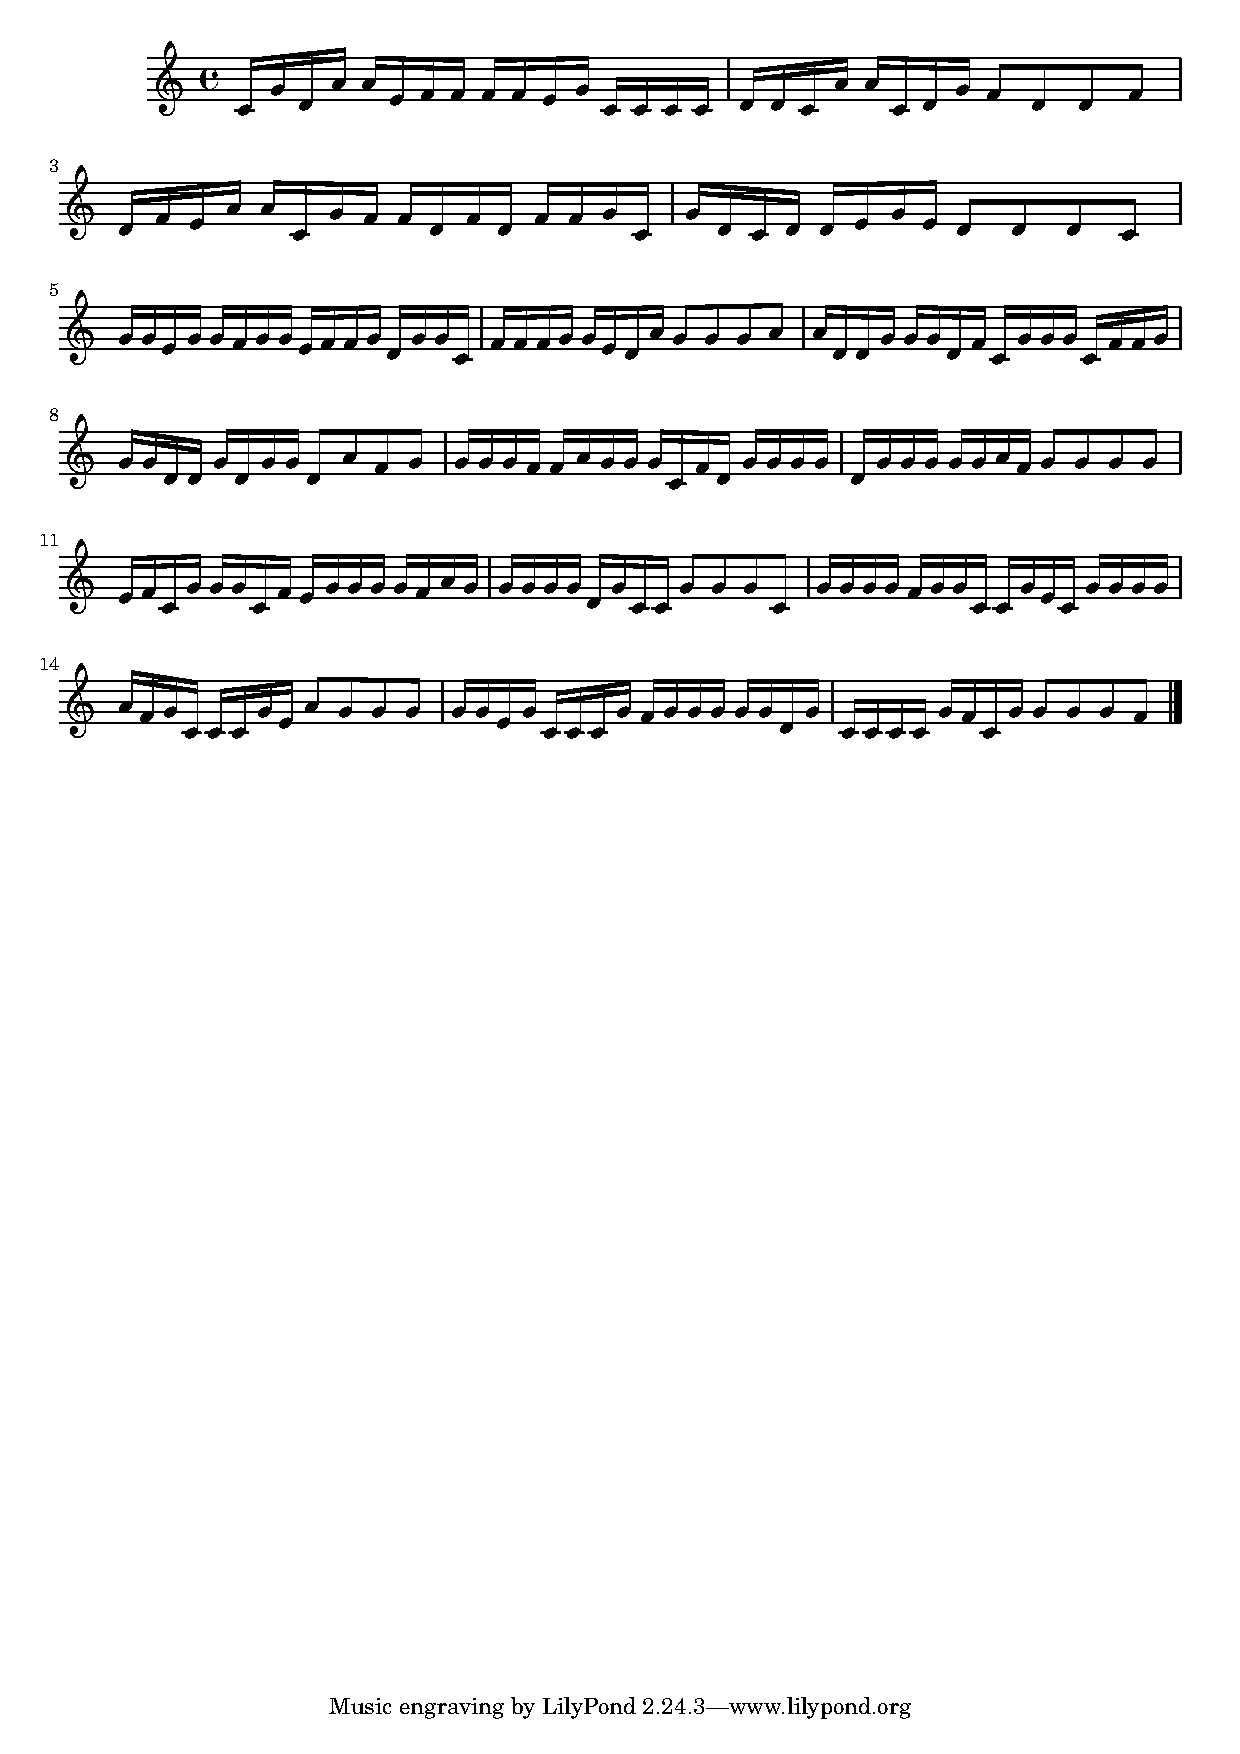
\includegraphics[trim=1cm 26.5cm 1cm 0.5cm, clip, scale=0.6]{dabby_melody_variation.pdf}
\caption{The new variation with melodic variation of Ah vous dirai-je, maman in the first 2 bars, generated by the Initial Condition $(1.01, 1, 1)$.} 
\label{fig:MVDabby}
\end{figure}

\section{Discussion}

This section explores the potential of Combination of Musical Variations from a Chaotic Mapping and Melodic Variation with Expanded Rhythm technique for generating musical variations. It analyzes the impact of this approach on the resulting variations compared to traditional melodic variation techniques. 

\subsection{Strengths of the Combined Approach}

The combined approach shows potential in generating interesting musical variations, as shown in the new variations with melodic variation of Pachelbel's Canon \cite{pachelbel_canon_2005} (Figure \ref{fig:NCND}) compared to the original melody (Figure \ref{fig:OCND}).

This method appears to be particularly effective for pieces with a larger range of musical pitches, as exemplified by Pachelbel's Canon. The additional pitches provide more material for the chaotic mapping and melodic variation techniques to manipulate, leading to richer and more diverse variations.

\begin{figure}
\centering
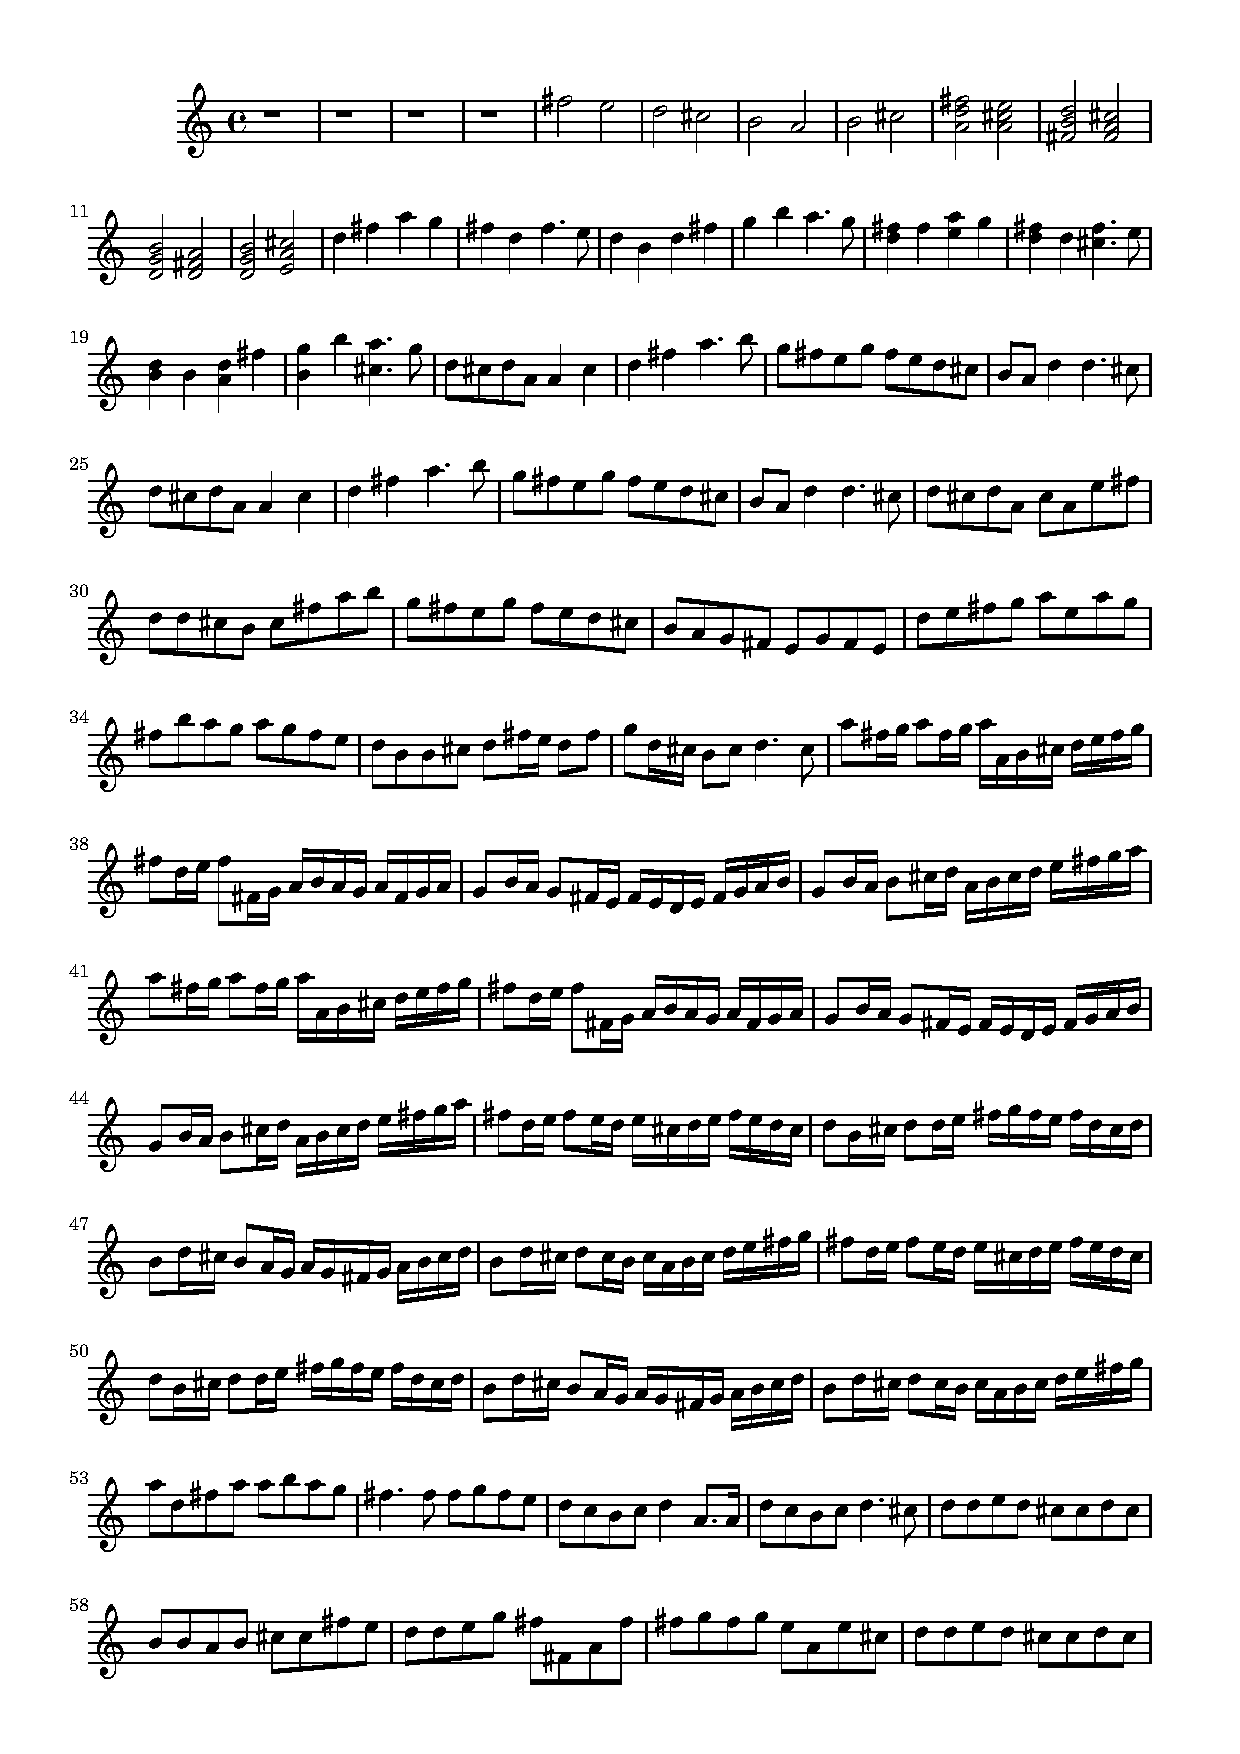
\includegraphics[trim=1cm 26.5cm 1cm 0.5cm, clip, scale=0.6]{Original_CND.pdf}
\caption{The original of Pachelbel's Canon in the first 10 bars.} 
\label{fig:OCND}
\end{figure}

\begin{figure}
\centering
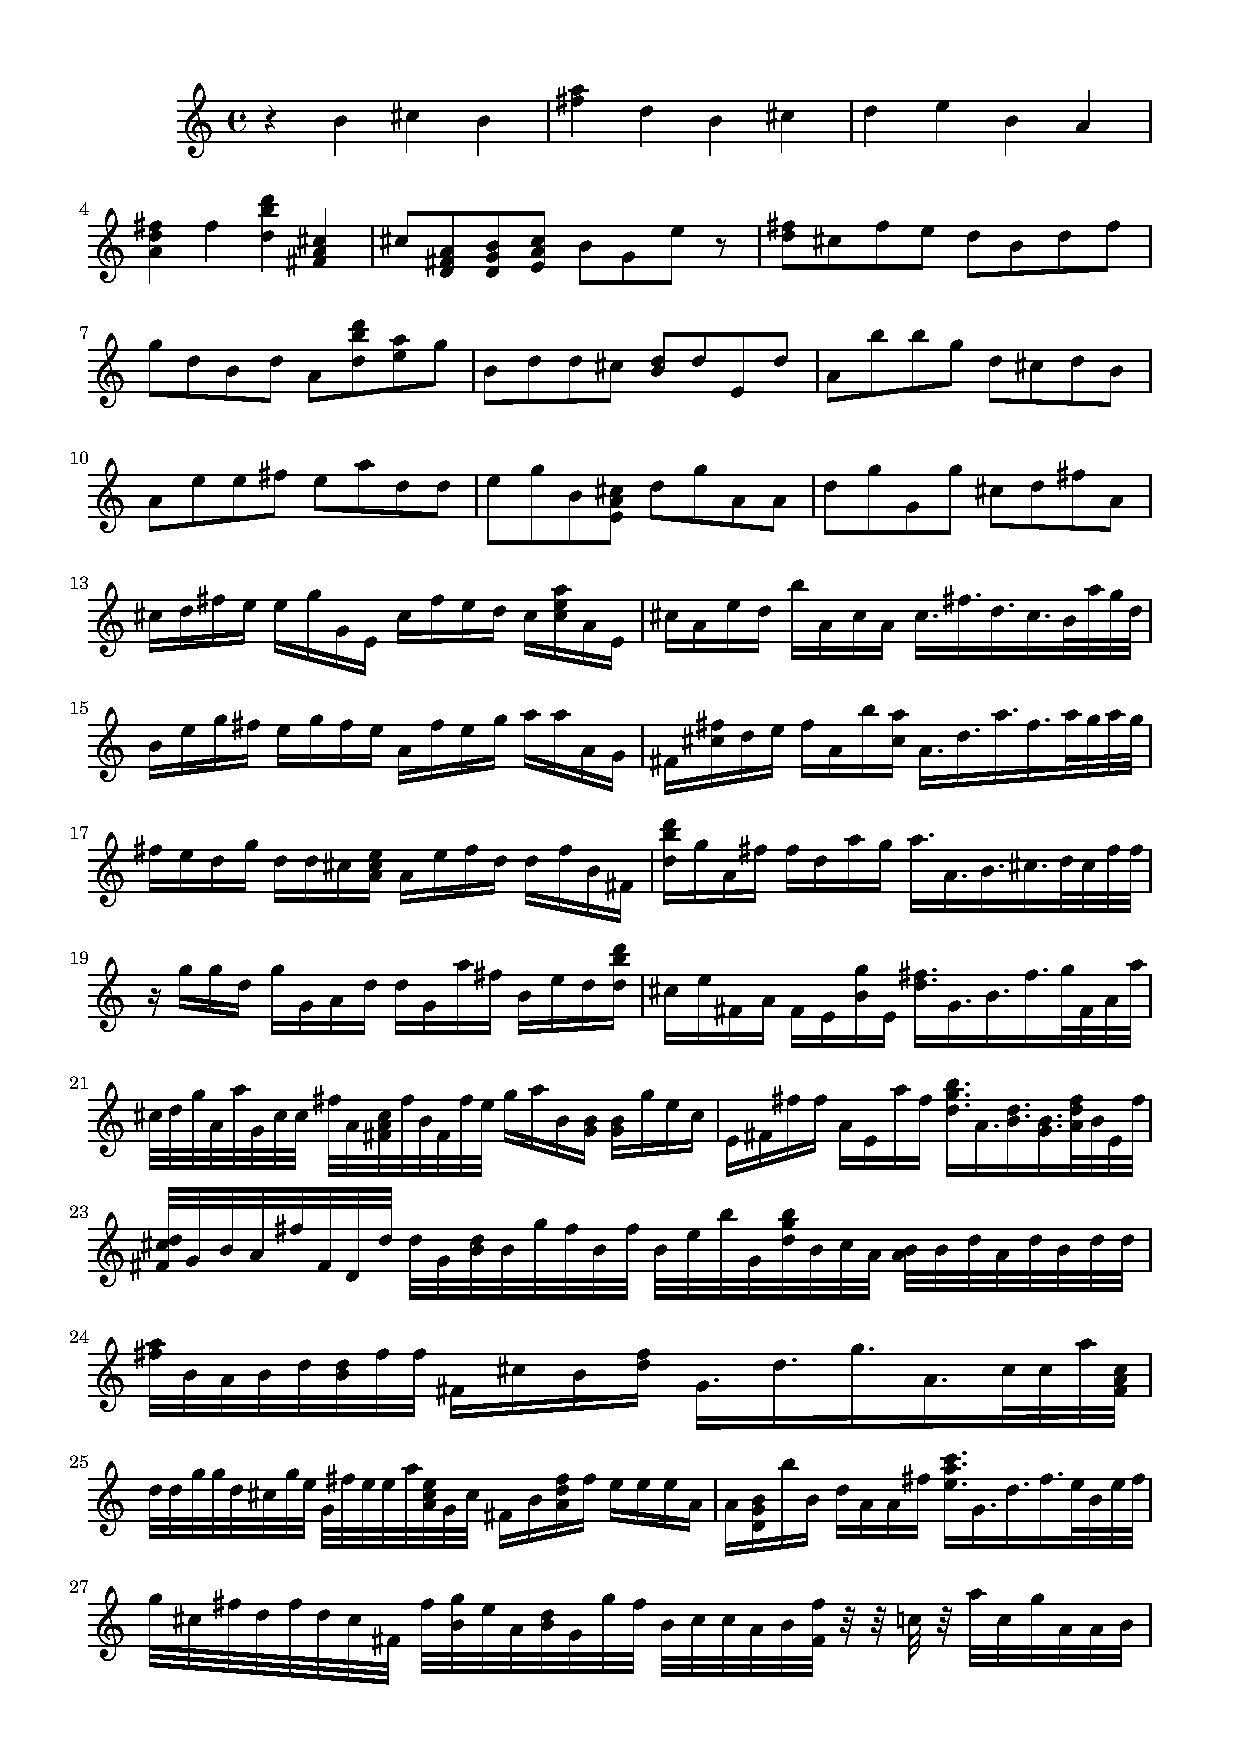
\includegraphics[trim=1cm 20.3cm 1cm 0.5cm, clip, scale=0.6]{New_CND.pdf}
\caption{The new variation with melodic variation of Pachelbel's Canon in the first 10 bars (including 2 additional bars at the end of the 10th bar), generated by the Initial Condition $(0.99, 0.99, 0.99)$.} 
\label{fig:NCND}
\end{figure}

\subsection{Weaknesses of the Combined Approach}

Let's consider the music sheet for Vanessa Carlton's A Thousand Miles (Figure \ref{fig:OATM}) and the new variation with melodic variation (Figure \ref{fig:NATM}). This result shows that using music sheets with too many musical note durations can lead to new variations with melodies that are difficult to play and listen to. This is a major weakness of this method.

\begin{figure}
\centering
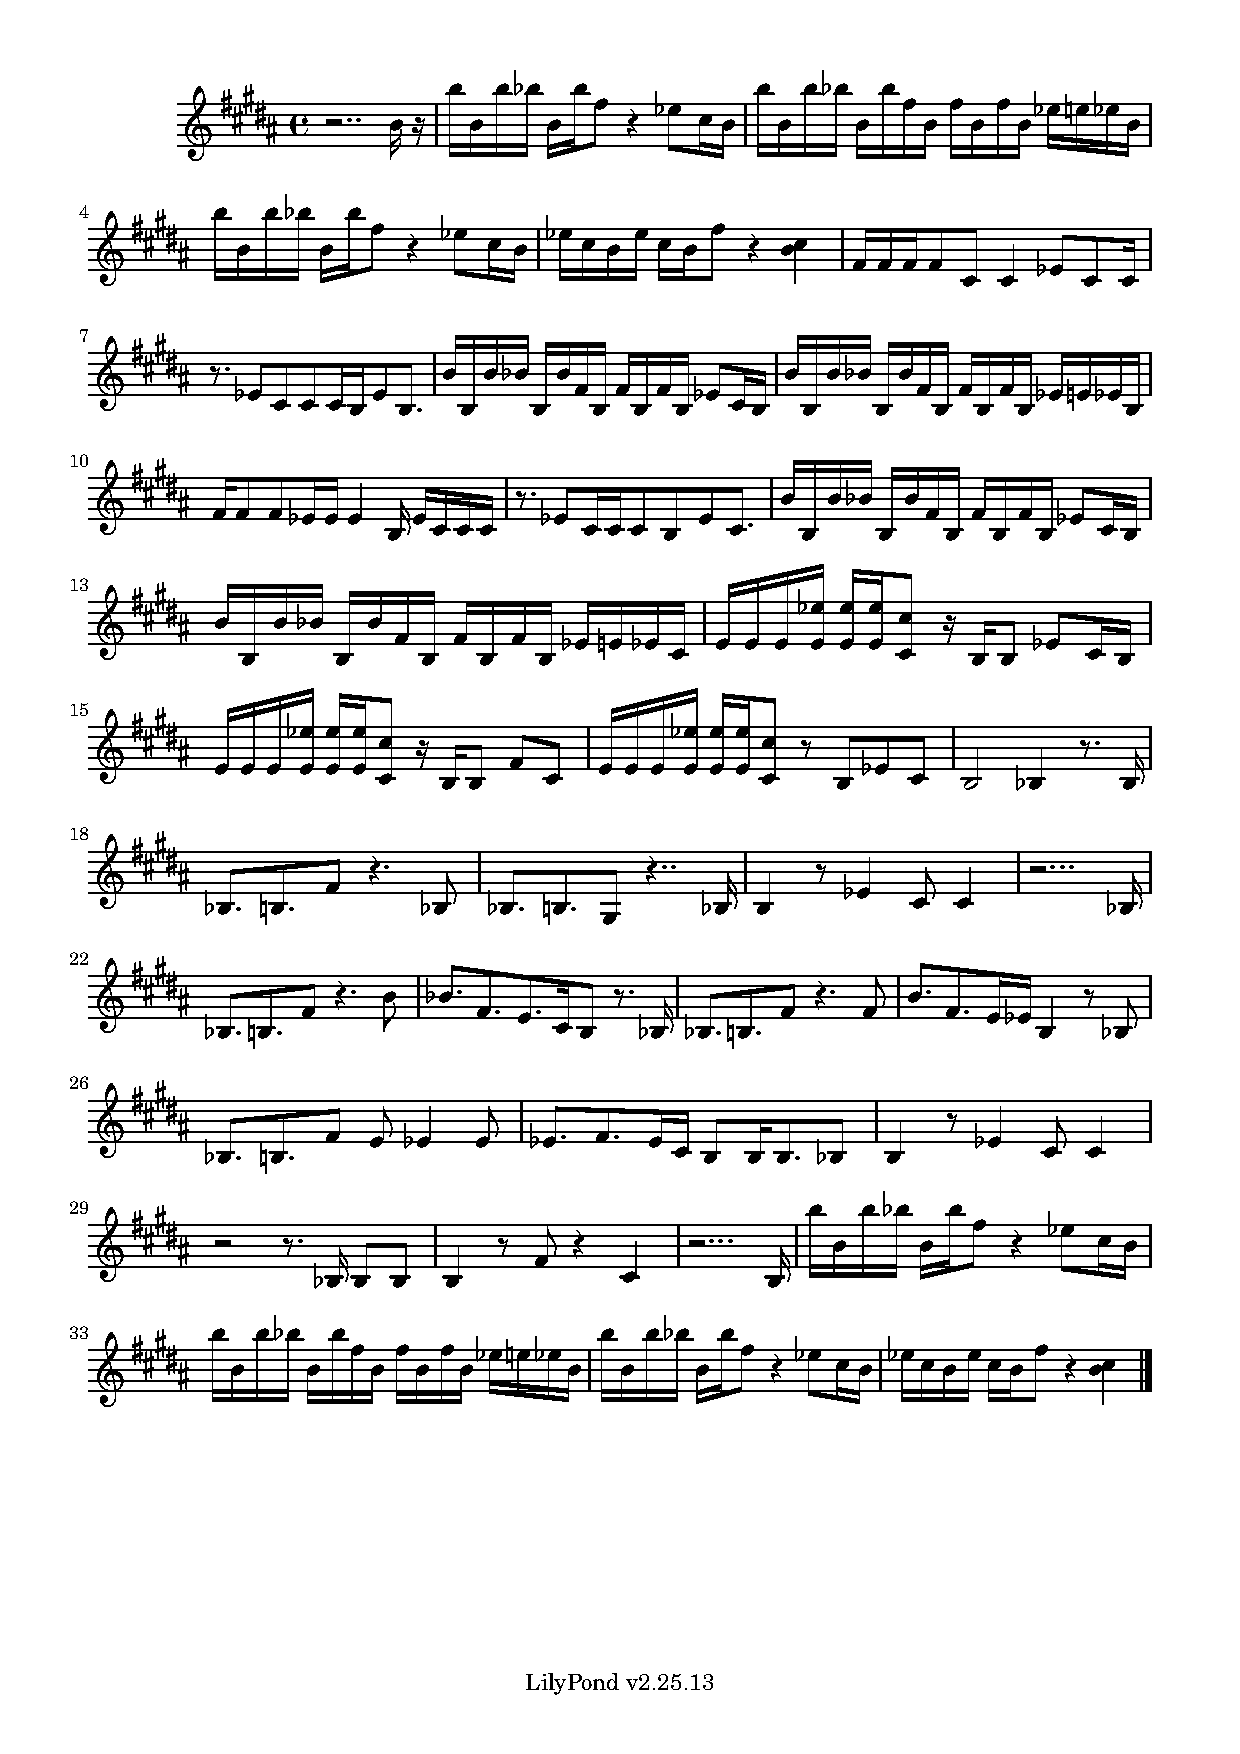
\includegraphics[trim=1cm 26.5cm 1cm 0.5cm, clip, scale=0.6]{Original_ATM.pdf}
\caption{The original of Vanessa Carlton - A Thousand Miles in the first 3 bars.} 
\label{fig:OATM}
\end{figure}

\begin{figure}
\centering
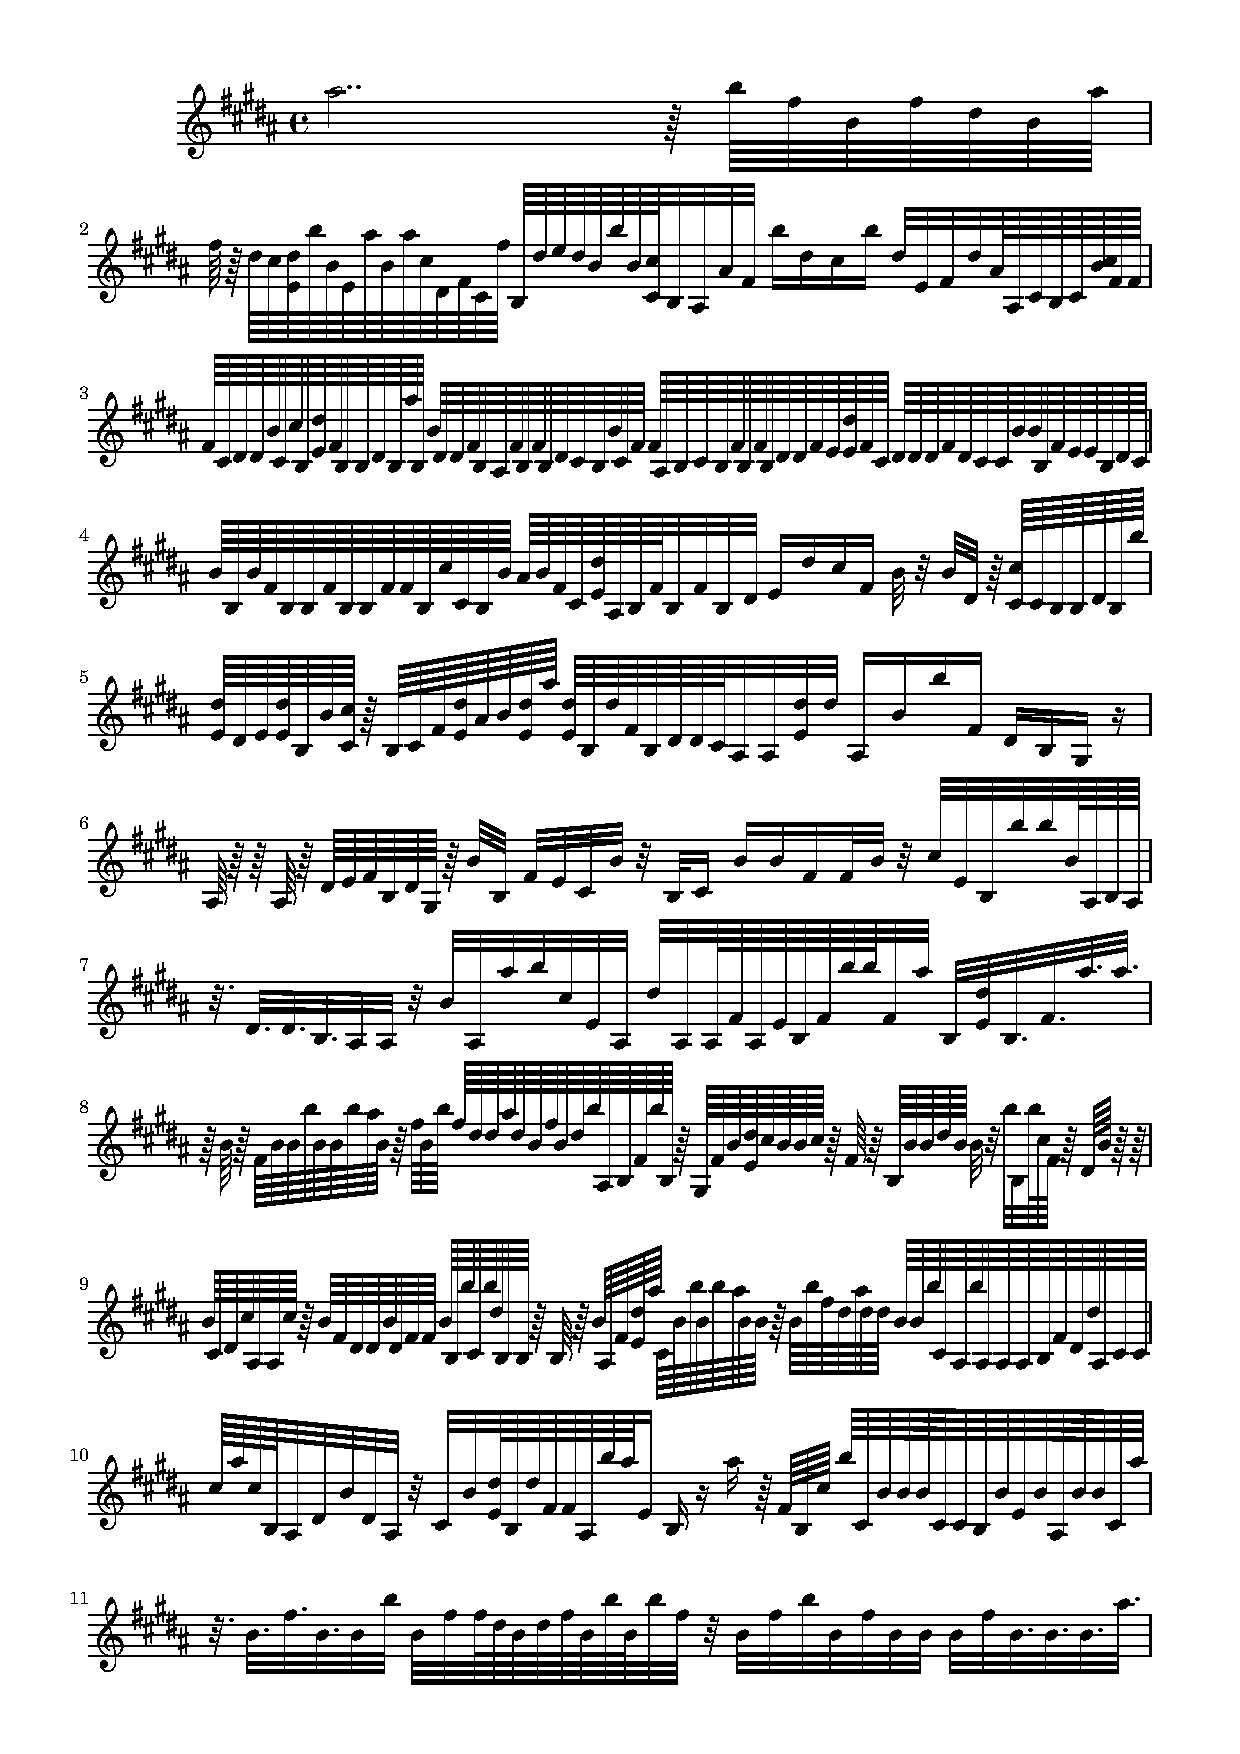
\includegraphics[trim=1cm 21.5cm 1cm 0.5cm, clip, scale=0.6]{New_ATM.pdf}
\caption{The new variation with melodic variation of Vanessa Carlton - A Thousand Miles in the first 3 bars, generated by the Initial Condition $(0.99, 0.99, 0.99)$.} 
\label{fig:NATM}
\end{figure}

\subsection{Limitations and Considerations}

Further evaluation with a wider range of musical pieces is necessary to determine the generalizability of these observations. The effectiveness of the combined approach might vary depending on the musical style and characteristics of the original piece.

The computational complexity of the chaotic mapping technique should also be considered. While it offers a powerful approach for variation, it might require more processing power compared to simpler melodic variation methods.

\subsection{Future Directions}

Exploring different parameters and configurations within the chaotic mapping and melodic variation techniques could potentially lead to a wider range of variation styles and outcomes.

Investigating methods for user control over the variation process would be valuable. This could allow musicians to tailor the generated variations to their specific creative goals.

Integrating this combined approach into music composition tools could provide composers with a valuable tool for generating new musical ideas and exploring creative possibilities.

\section{Conclusion}

The proposed method, leveraging the power of chaotic systems, offers a promising approach to music composition, addressing the limitations of existing AI techniques and providing composers with a tool to generate novel, unpredictable, and diverse musical compositions while reducing computational resource demands. This method has the potential to stimulate creativity, alleviate composer's burnout, and expand the boundaries of musical expression, paving the way for a new era of music creation driven by chaos and innovation.

\begin{figure}
\centering
\begin{subfigure}{0.45\textwidth}
  \centering
  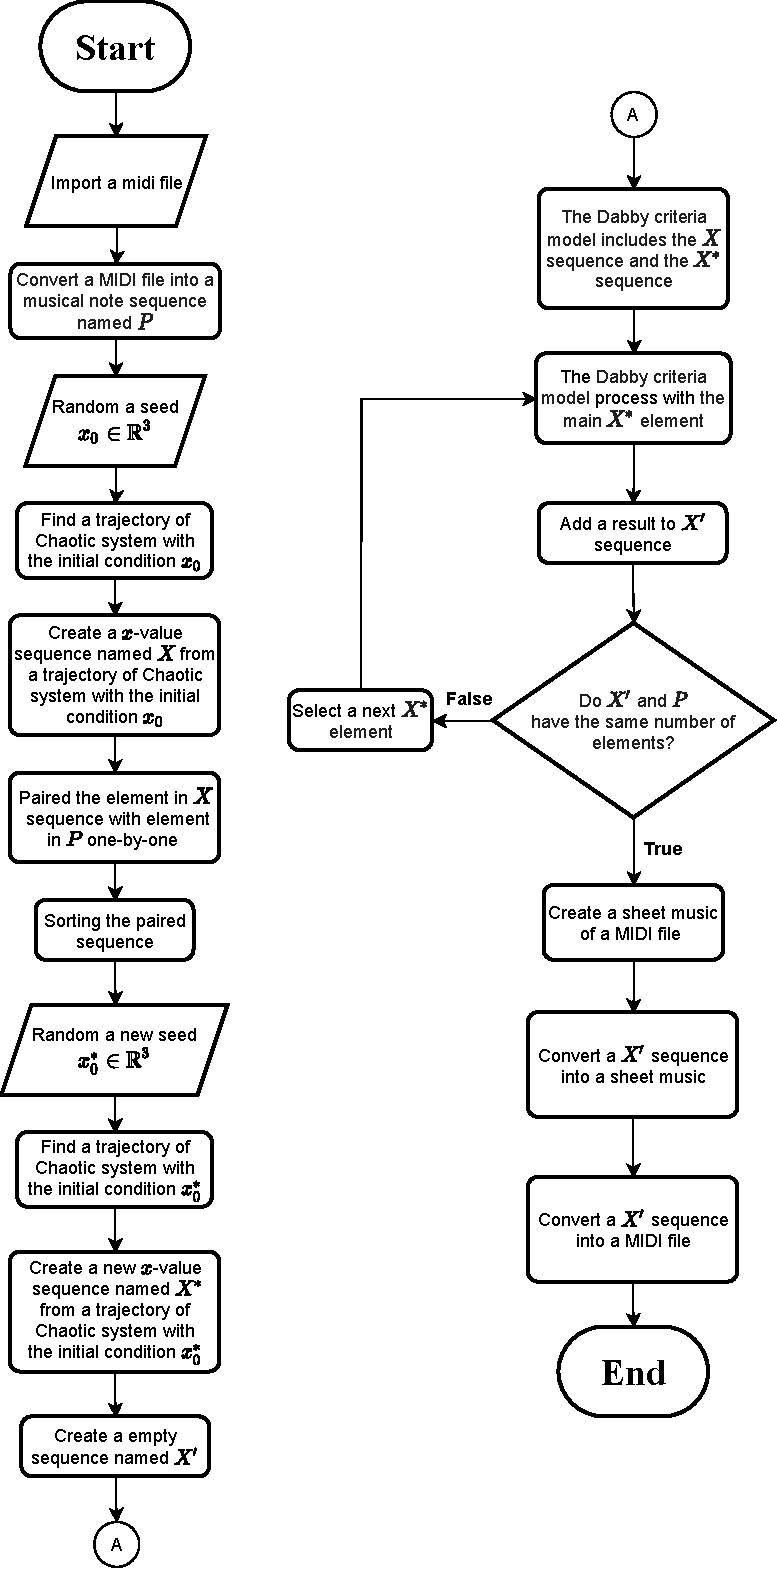
\includegraphics[scale=0.55]{Dabby_process.pdf}
  \caption{Flowchart of musical variations from a chaotic mapping (Diana S. Dabby)}
\end{subfigure}
\begin{subfigure}{0.45\textwidth}
  \centering
  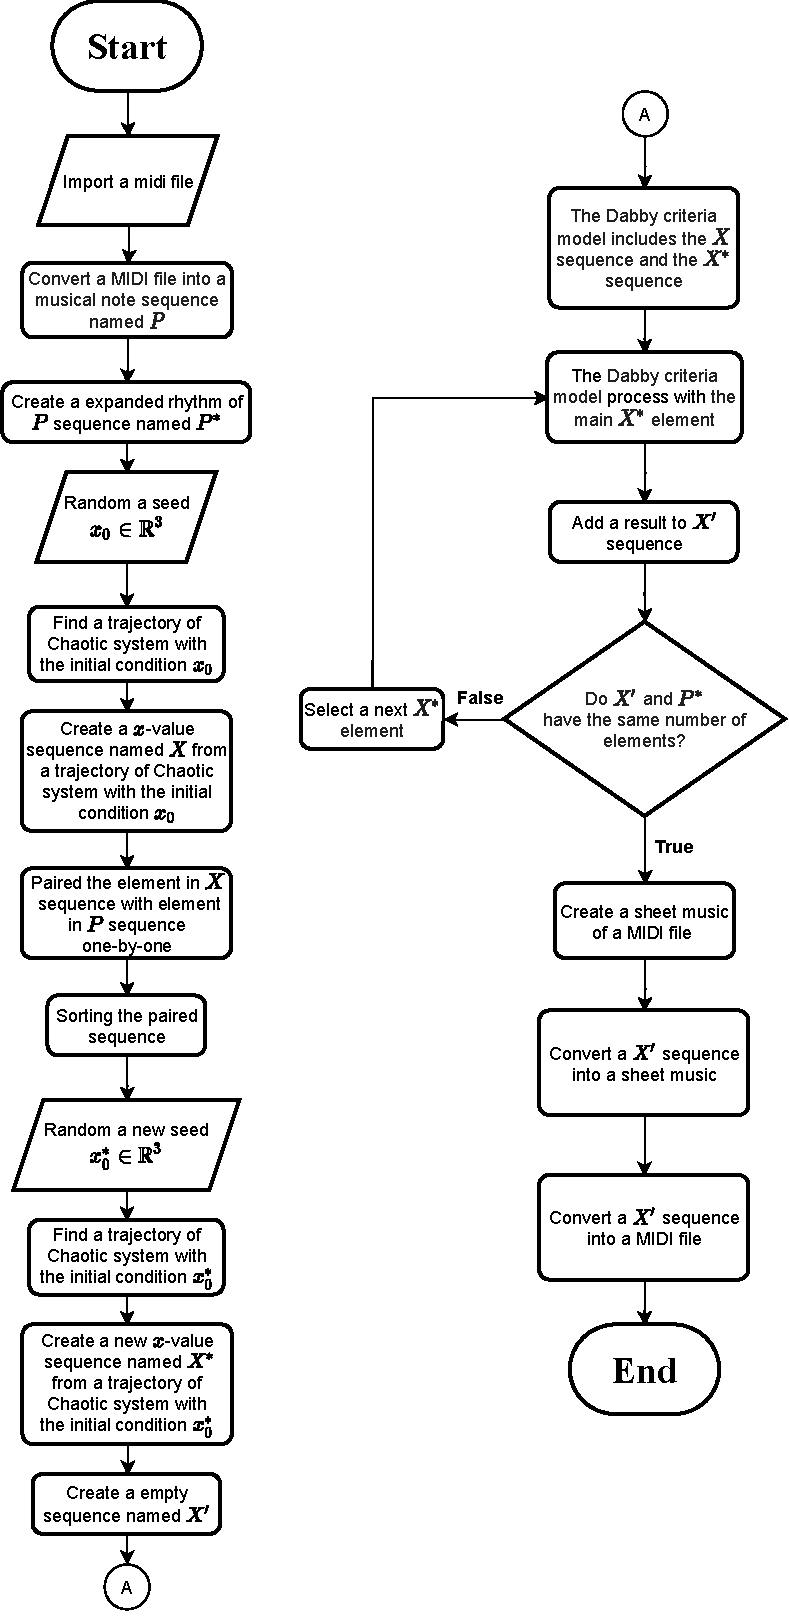
\includegraphics[scale=0.55]{Real_process.pdf}
  \caption{Flowchart of combining musical variations from a chaotic mapping (Diana S. Dabby) and melodic variation with expanded rhythm}
\end{subfigure}
\caption{Flowcharts of musical variations}
\label{fig:combined_flowcharts}
\end{figure}

\pagebreak

\printbibliography

\end{document}